\documentclass[final,t]{beamer}\usepackage[]{graphicx}\usepackage[]{color}
% maxwidth is the original width if it is less than linewidth
% otherwise use linewidth (to make sure the graphics do not exceed the margin)
\makeatletter
\def\maxwidth{ %
  \ifdim\Gin@nat@width>\linewidth
    \linewidth
  \else
    \Gin@nat@width
  \fi
}
\makeatother

\definecolor{fgcolor}{rgb}{0.345, 0.345, 0.345}
\makeatletter
\@ifundefined{AddToHook}{}{\AddToHook{package/xcolor/after}{\definecolor{fgcolor}{rgb}{0.345, 0.345, 0.345}}}
\makeatother
\newcommand{\hlnum}[1]{\textcolor[rgb]{0.686,0.059,0.569}{#1}}%
\newcommand{\hlstr}[1]{\textcolor[rgb]{0.192,0.494,0.8}{#1}}%
\newcommand{\hlcom}[1]{\textcolor[rgb]{0.678,0.584,0.686}{\textit{#1}}}%
\newcommand{\hlopt}[1]{\textcolor[rgb]{0,0,0}{#1}}%
\newcommand{\hlstd}[1]{\textcolor[rgb]{0.345,0.345,0.345}{#1}}%
\newcommand{\hlkwa}[1]{\textcolor[rgb]{0.161,0.373,0.58}{\textbf{#1}}}%
\newcommand{\hlkwb}[1]{\textcolor[rgb]{0.69,0.353,0.396}{#1}}%
\newcommand{\hlkwc}[1]{\textcolor[rgb]{0.333,0.667,0.333}{#1}}%
\newcommand{\hlkwd}[1]{\textcolor[rgb]{0.737,0.353,0.396}{\textbf{#1}}}%
\let\hlipl\hlkwb

\usepackage{framed}
\makeatletter
\newenvironment{kframe}{%
 \def\at@end@of@kframe{}%
 \ifinner\ifhmode%
  \def\at@end@of@kframe{\end{minipage}}%
  \begin{minipage}{\columnwidth}%
 \fi\fi%
 \def\FrameCommand##1{\hskip\@totalleftmargin \hskip-\fboxsep
 \colorbox{shadecolor}{##1}\hskip-\fboxsep
     % There is no \\@totalrightmargin, so:
     \hskip-\linewidth \hskip-\@totalleftmargin \hskip\columnwidth}%
 \MakeFramed {\advance\hsize-\width
   \@totalleftmargin\z@ \linewidth\hsize
   \@setminipage}}%
 {\par\unskip\endMakeFramed%
 \at@end@of@kframe}
\makeatother

\definecolor{shadecolor}{rgb}{.97, .97, .97}
\definecolor{messagecolor}{rgb}{0, 0, 0}
\definecolor{warningcolor}{rgb}{1, 0, 1}
\definecolor{errorcolor}{rgb}{1, 0, 0}
\makeatletter
\@ifundefined{AddToHook}{}{\AddToHook{package/xcolor/after}{
\definecolor{shadecolor}{rgb}{.97, .97, .97}
\definecolor{messagecolor}{rgb}{0, 0, 0}
\definecolor{warningcolor}{rgb}{1, 0, 1}
\definecolor{errorcolor}{rgb}{1, 0, 0}
}}
\makeatother
\newenvironment{knitrout}{}{} % an empty environment to be redefined in TeX

\usepackage{alltt}
\mode<presentation>{\usetheme{I6dv}}

% settings
\setbeamerfont{itemize}{size=\normalsize}
\setbeamerfont{itemize/enumerate body}{size=\normalsize}
\setbeamerfont{itemize/enumerate subbody}{size=\normalsize}
\setbeamertemplate{caption}[numbered]

% packages
\usepackage{xcolor}
\usepackage{times}
\usepackage{amsmath,amsthm, amssymb, latexsym}
\usepackage{exscale}
\usepackage{subfig}
\usepackage{booktabs, array}
\usepackage{tabularx}
\usepackage[english]{babel}
\usepackage[latin1]{inputenc}
\usepackage[orientation=landscape,size=custom,width=21.59,height=27.94,scale=0.45]{beamerposter} % in cm, equal to 8.5" wide x 11" high
\usepackage{color, colortbl}
% \usepackage[printwatermark]{xwatermark}
\usepackage{graphicx}
\usepackage{tikz}

% % for watermark using tikz
% \newsavebox\mybox
% \savebox\mybox{\tikz[color=red,opacity=0.3]\node{DRAFT};}
% \newwatermark*[
%   allpages,
%   angle=45,
%   scale=6,
%   xpos=-20,
%   ypos=15
% ]{\usebox\mybox}

% \setcounter{figure}{1}
\renewcommand{\arraystretch}{1.35}



\title{\Large 2021 Tampa Bay Water Quality Assessments}
\author{\normalsize A Tampa Bay Estuary Program Initiative to Maintain and Restore the Bay's Seagrass Resources}
\IfFileExists{upquote.sty}{\usepackage{upquote}}{}
\begin{document}

\begin{frame}

\vspace{-0.4cm} %spacing for block distance from header
\begin{columns}[t]

%%%%%%%%%%%%%%
% left
%%%%%%%%%%%%%%
\begin{column}{.2\linewidth}

\vspace{-0.2in}


\begin{figure}
\centerline{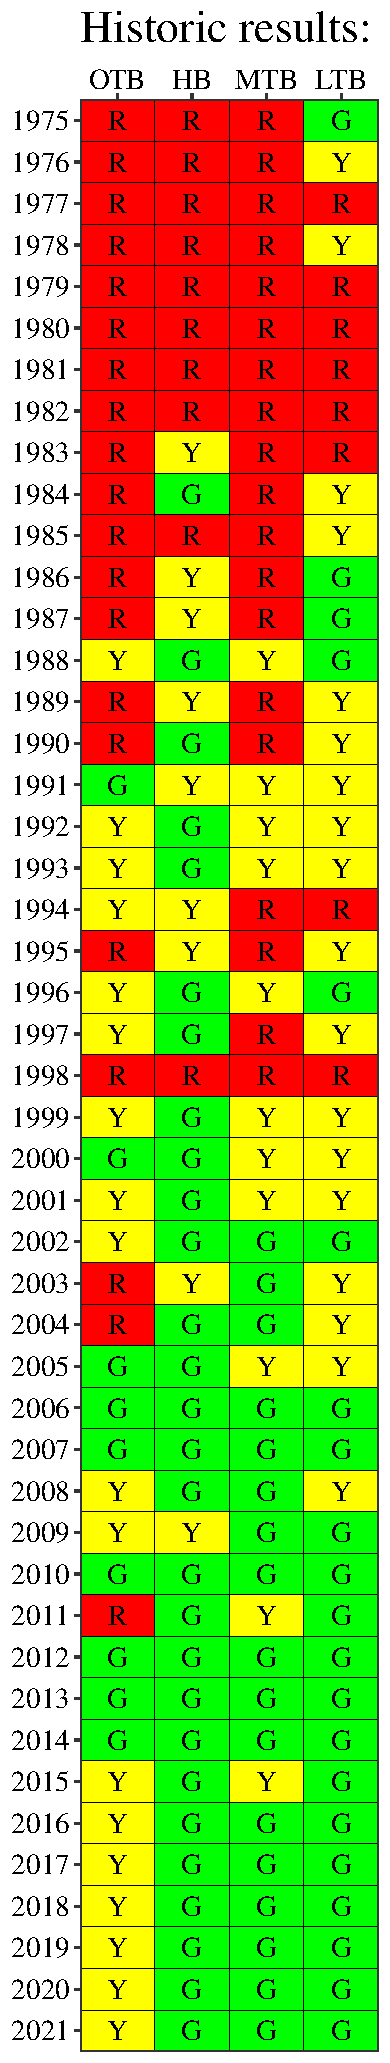
\includegraphics[trim = 0cm 0cm 0cm 0cm, width=1.1\linewidth]{figure/attainmat.pdf}}
\caption{\footnotesize Decision matrix results for 1975 to 2021 (April, May data missing for 2020).}
\label{fig:attainmat}
\end{figure}

\end{column}

%%%%%%%%%%%%%%
% right
%%%%%%%%%%%%%%
\begin{column}{.79\linewidth}

\begin{block}{Background}
\begin{minipage}{0.5\textwidth}
\vspace{-0.2in}
\footnotesize
Light availability to seagrass is the guiding paradigm for TBEP's Nitrogen Management Strategy. Because excessive nitrogen loads to the bay generally lead to increased algae blooms (higher chlorophyll-a levels) (Figure \ref{fig:nitro}) and reduce light penetration to seagrass, an evaluation method was developed to assess whether load reduction strategies are achieving desired water quality results (i.e. reduced chlorophyll-a concentrations and increased water clarity).
\end{minipage}
\hspace{0.1in}
\begin{minipage}{0.45\textwidth}
\begin{figure}
\includegraphics[width=0.9\textwidth]{www/nitro.jpg}
\caption{\footnotesize Seagrass restoration with N management.}
\label{fig:nitro}
\end{figure}
\end{minipage}
\vspace{-0.2in}
\end{block}

\begin{block}{Decision Support Approach}
\begin{minipage}{0.5\textwidth}
\footnotesize
Year to year algae abundance (measured as chlorophyll-a concentrations) and visible light penetration through the water column (secchi disk depth visibility) have been identified as critical water quality indicators in Tampa Bay. Tracking the attainment of bay segment specific targets for these indicators provides the framework for developing and initiating bay management actions. TBEP management actions adopted in response to the annually-assessed decision support results are shown to the right.
\end{minipage}
\hspace{0.01in}
\begin{minipage}{0.45\textwidth}
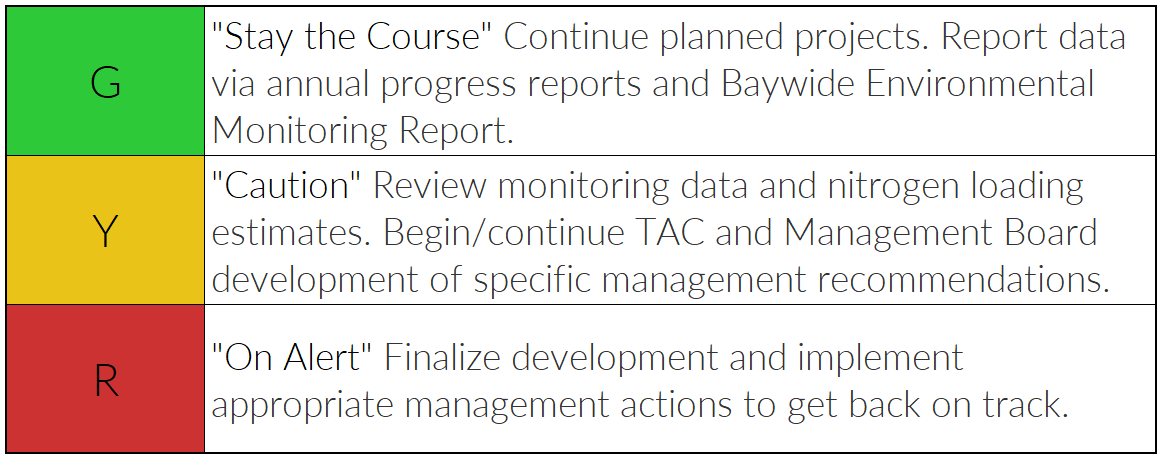
\includegraphics[width=1\textwidth]{www/stoplight.PNG}
\end{minipage}
\end{block}

\begin{block}{2021 Decision Matrix Results}
\vspace{-0.1in}
\begin{minipage}{0.45\textwidth}
\footnotesize
Water quality (chlorophyll-a and light penetration) remained supportive of seagrass in Hillsborough Bay (HB), Middle Tampa Bay (MTB), and Lower Tampa Bay (LTB)(Table \ref{tab:segtab}, Figure \ref{fig:thrplot}). The nuisance alga, \textit{Pyrodinium bahamense}, was again reported in Old Tampa Bay (OTB) during June - Sept 2020, contributing to a large magnitude chlorophyll-a exceedance that has persisted for a long duration (6 yrs). However, it should be noted that effective light penetration was still observed to be supportive of seagrass in all bay segments, including OTB (Table \ref{tab:segtab}).
\end{minipage}
\hspace{0.1in}
\begin{minipage}{0.5\textwidth}
\footnotesize
%latex.default(tab, file = "", caption = cap.val, caption.loc = "top",     cgroup = cgrps, n.cgroup = c(2, 2), rowlabel = "Segment",     colheads = c(maxyr, "target", maxyr, "target"), label = "tab:segtab",     col.just = c("c", "c", "c", "c"), table.env = F)%
\begin{table}[!tbp]
\caption{{\footnotesize Water quality outcomes for 2021.}\label{tab:segtab}} 
\begin{center}
\begin{tabular}{lccccc}
\hline\hline
\multicolumn{1}{l}{\bfseries Segment}&\multicolumn{2}{c}{\bfseries Chl-a (ug/L)}&\multicolumn{1}{c}{\bfseries }&\multicolumn{2}{c}{\bfseries Light Penetration (m$^{-1}$)}\tabularnewline
\cline{2-3} \cline{5-6}
\multicolumn{1}{l}{}&\multicolumn{1}{c}{2021}&\multicolumn{1}{c}{target}&\multicolumn{1}{c}{}&\multicolumn{1}{c}{2021}&\multicolumn{1}{c}{target}\tabularnewline
\hline
\cellcolor{yellow}OTB&$~9.3$&$~8.5$&&$0.74$&$0.83$\tabularnewline
\cellcolor{green}HB&$10.4$&$13.2$&&$1.03$&$1.58$\tabularnewline
\cellcolor{green}MTB&$~5.2$&$~7.4$&&$0.58$&$0.83$\tabularnewline
\cellcolor{green}LTB&$~3.4$&$~4.6$&&$0.62$&$0.63$\tabularnewline
\hline
\end{tabular}\end{center}
\end{table}

\end{minipage}

\end{block}

\vspace{-0.55in}

\begin{columns}[t]



\begin{column}{0.585\textwidth}
\vspace{-0.4cm}
\begin{figure}[htbp]
% \hspace*{2cm}
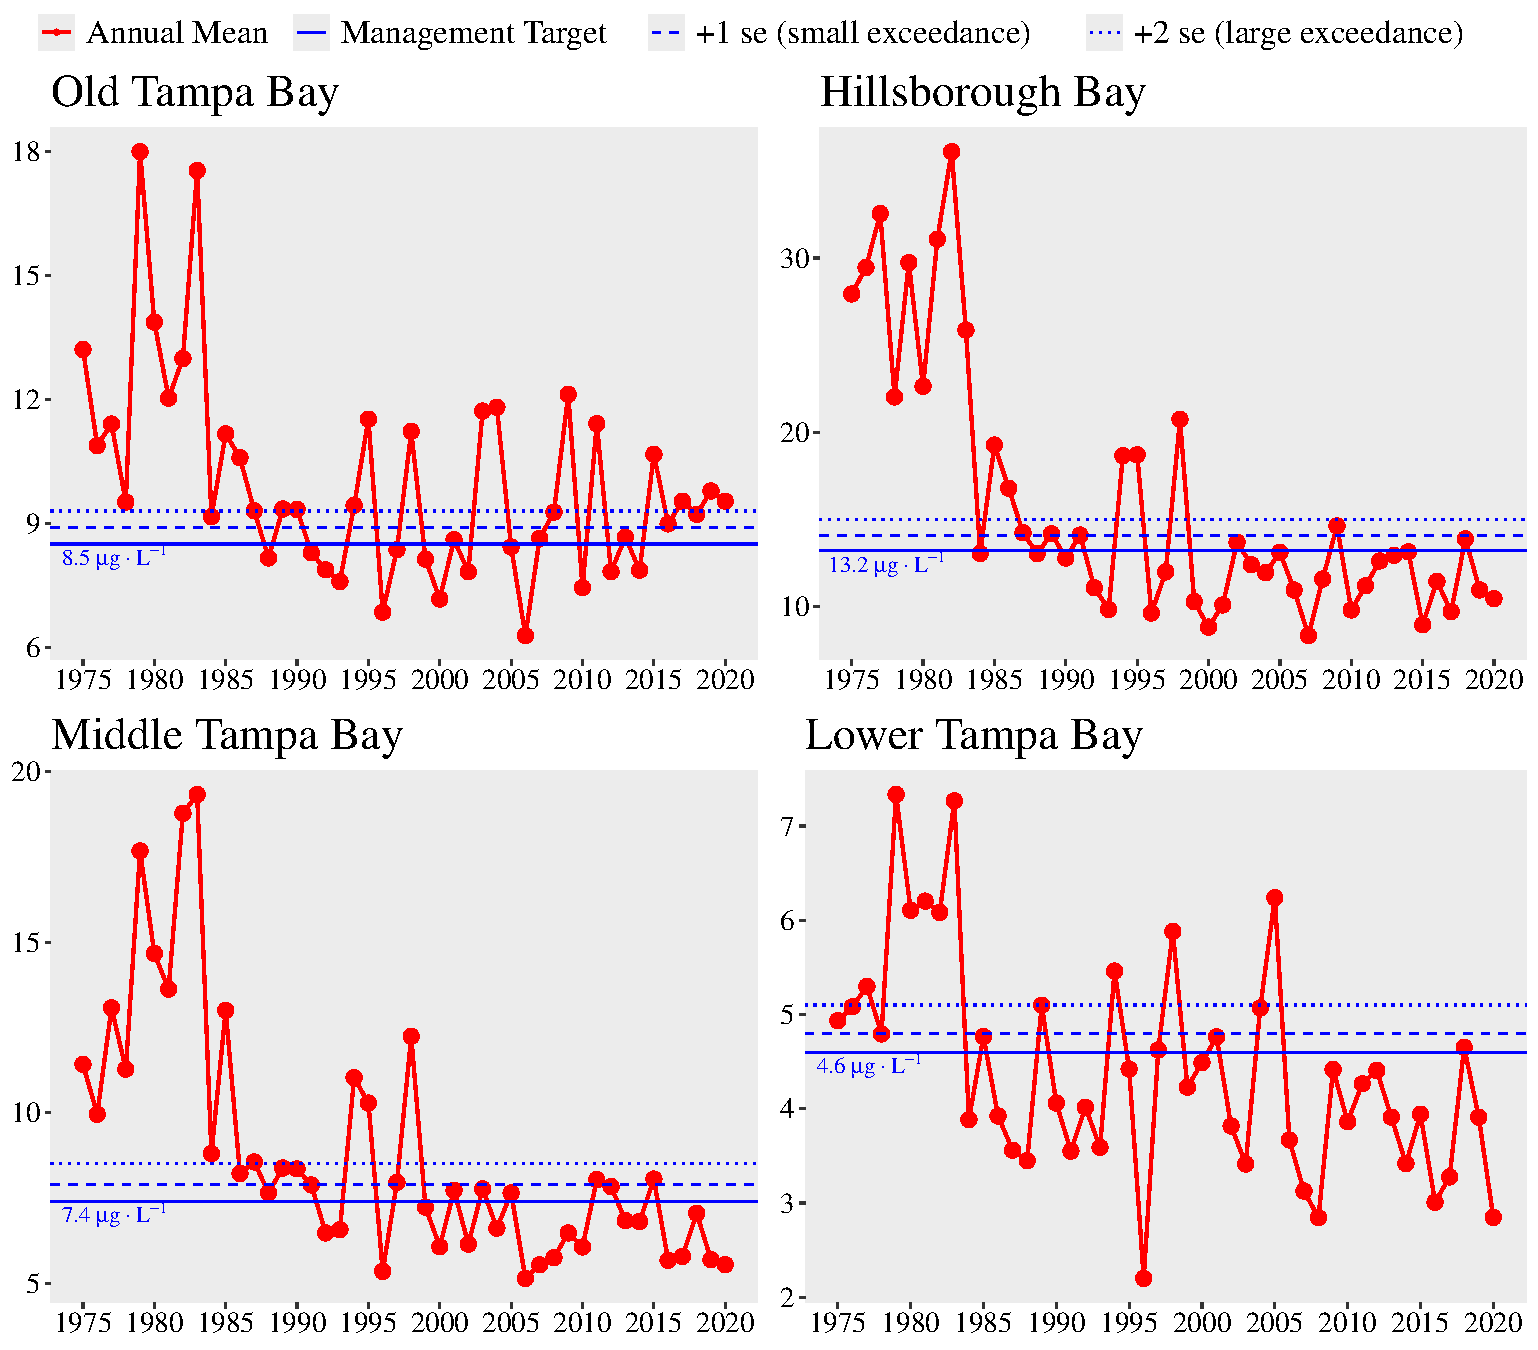
\includegraphics[trim = 0cm 0cm 0cm 0cm, width=1.09\linewidth]{figure/thrplot.pdf}
\caption{\footnotesize Historic chlorophyll-a annual averages for the four bay segments.}
\label{fig:thrplot}
\end{figure}

\end{column}



\begin{column}{0.37\textwidth}

\begin{figure}
\centerline{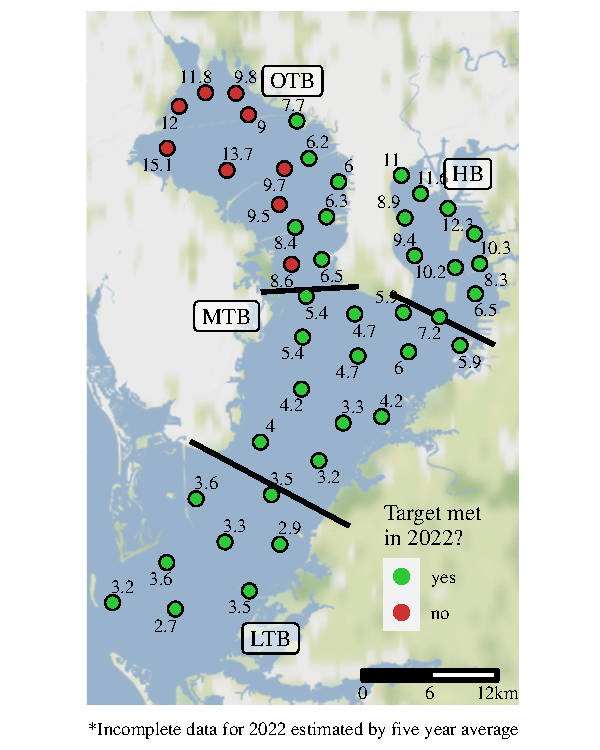
\includegraphics[trim = 0cm 0cm 0cm -1.25cm, width=1.1\linewidth]{figure/sitemap.pdf}}
\caption{\footnotesize Chlorophyll attainment outcomes by site for 2021.}
\label{fig:sitemap}
\end{figure}

\end{column}

\end{columns}

\vspace{-0.4cm}

\tiny \textit{\textbf{Note}: Continuing water quality monitoring support provided by the Environmental Protection Commission of Hillsborough County.  Consulting support provided by Janicki Environmental, Inc.  Full methods in Janicki et al. 2000. \href{https://drive.google.com/file/d/1XMULU8w4syWcSv_ciOUOhnC_G4xt6GIF/view?usp=drivesdk}{TBEP Technical Report \#04-00}. Points in map above show site-specific attainment of a bay segment target and are for reference only.} \\

\end{column}

\end{columns}

\end{frame}

\end{document}
